\documentclass[../Práctica.root.tex]{subfiles}

% Para usar en el ejercicio 9.2.7
% Define un comando que dibuja dos circulos pegados, uno de color #1 y el otro #2
\tikzset{
    pics/molecula/.style args={#1/#2}{
        code={
            \filldraw[fill=#1] circle[radius=0.25] node(x){};
            \filldraw[fill=#2] (x) +(0.5,0) circle[radius=0.25];
        }
    }
}

% Kc = \frac{[C]^c\cdot[D]^d}{[A]^a\cdot[B]^b}

\begin{document}
\section{Unidad 9}
\subsection{Bloque 1}
\begin{enumerate}
    \item[1.] En un recipiente se produce una reacción química hasta alcanzar el equilibrio. Indiquen si
          las siguientes afirmaciones son correctas (C) o incorrectas (I). Justifiquen las respuestas.
          \begin{enumerate}
              \item En el equilibrio, la concentración de una de las sustancias es cero.
              \item A nivel submicroscópico, la reacción química se sigue produciendo en ambos
                    sentidos. \checkmark
              \item Una vez alcanzado el equilibrio, la velocidad de la reacción directa es mayor que la
                    velocidad de la reacción inversa.
              \item La reacción es irreversible.
              \item En el equilibrio se encuentran presentes todas las especies químicas. \checkmark
              \item En el equilibrio, la concentración de todas las especies químicas es la misma.
              \item El valor de la constante de equilibrio depende solamente de la temperatura. \checkmark
          \end{enumerate}

    \item[4.] En un matraz de \SI{1,00}{\dm\cubed} a \SI{327}{\celsius}, se produce la reacción entre monóxido de nitrógeno y
          oxígeno, representada por la siguiente ecuación:
          \[ 2 NO \eg + O_2 \eg \llra 2 NO_2 \eg \]
          Una vez alcanzado el equilibrio, el sistema está formado por: \SI{1,80e-4}{\mole} de $NO$,
          \SI{3,00e-3}{\mole} de $O_2$ y \SI{7,90e-3}{\mole} de $NO_2$. Calculen el valor de $Kc$ a \SI{327}{\celsius}.
          \[ Kc = \frac{[C]^c\cdot[D]^d}{[A]^a\cdot[B]^b} \]
          \[ Kc = \frac{ [NO_2]^2 }{ [NO]^2 \cdot [O_2] } \]
          \[ Kc = \frac{ [\num{7,90e-3}]^2 }{ [\num{1,80e-4}]^2 \cdot \num{3,00e-3} } \]
          \[ \boxed{Kc = \num{6,42E5}} \]

    \item[6.] En un recipiente de \SI{1,50}{\dm\cubed} a determinada temperatura, se introducen \SI{1,20}{\mole} de $SO_2$ y
          \SI{2,25}{\mole} de $O_2$. Una vez alcanzado el equilibrio, el sistema está formado por
          \SI{0,360}{\mole} de $SO_2$; \SI{1,83}{\mole} de $O_2$ y \SI{0,840}{\mole} de $SO_3$. La ecuación que representa el
          proceso es:
          \[ 2 SO_2 \eg + O_2 \eg \llra 2 SO_3 \eg \]
          \begin{enumerate}
              \item Calculen el valor de la constante de equilibrio a esa temperatura.
                    \[ Kc = \frac{[C]^c\cdot[D]^d}{[A]^a\cdot[B]^b} \]
                    \[ Kc = \frac{[SO_3]^2}{[SO_2]^2\cdot[O_2]} \]
                    \begin{align*}
                        [SO_2] & = \SI{0,360/1,5}{\mole\per\dm\cubed} & [O_2] & = \SI{1,83/1,5}{\mole\per\dm\cubed} & [SO_3] & = \SI{0,84/1,5}{\mole\per\dm\cubed} \\
                        [SO_2] & = \SI{0,240}{\MR}                    & [O_2] & = \SI{1,22}{\MR}                    & [SO_3] & = \SI{0,56}{\MR}
                    \end{align*}
                    \[ Kc
                        = \frac{\num{0,56}^2}
                        {\num{0,240}^2\cdot\num{1,22}}
                    \]
                    \[ \boxed{Kc = \num{4,46}} \]
              \item Completen el siguiente cuadro con la información solicitada.
                    \begin{center}
                        \begin{tabular}{l|c c c c c}
                                                                 & $2 SO_2 \eg$      & + & $O_2 \eg$        & \llra & $2 SO_3 \eg$      \\
                            \hline
                            Cantidad inicial                     & \SI{1,20}{\mole}  &   & \SI{2,25}{\mole} &       & \SI{0}{\mole}     \\
                            Cantidad que reacciona               & \SI{0,84}{\mole}  &   & \SI{0,42}{\mole} &       & \SI{0}{\mole}     \\
                            Cantidad que se forma                & \SI{0}{\mole}     &   & \SI{0}{\mole}    &       & \SI{0,84}{\mole}  \\
                            Cantidad en equilibrio               & \SI{0,360}{\mole} &   & \SI{1,83}{\mole} &       & \SI{0,840}{\mole} \\
                            Concentración molar en el equilibrio & \SI{0,240}{\MR}   &   & \SI{1,22}{\MR}   &       & \SI{0.560}{\MR}
                        \end{tabular}
                    \end{center}
          \end{enumerate}

    \item[10.] En un matraz de \SI{4,00}{\dm\cubed}, a \SI{250}{\celsius}, se introducen \SI{1,00}{\mole} de $NOBr \eg$;
          \SI{1,00}{\mole} de $NO \eg$ y \SI{1,00}{\mole} de $Br_2 \eg$. El valor de $Kc( 523 K)$ es de \num{2,00} y la ecuación % Qué significa "Kc( 523 K)"?
          que representa la reacción es:
          \[ 2 NOBr \eg \llra 2 NO \eg + Br_2 \eg \]
          Indiquen:
          \begin{enumerate}
              \item si el sistema se encuentra en equilibrio o, de lo contrario, en qué sentido evoluciona
                    para alcanzarlo;
                    \[ Qc = \frac{[C]^c\cdot[D]^d}{[A]^a\cdot[B]^b} \]
                    \[ Qc = \frac{[NO]^2\cdot[Br_2]}{[NOBr]^2} \]
                    \begin{align*}
                        [NOBr] & = \SI{1,00/4,00}{\mole\per\dm\squared} & [NO] & = \SI{1,00/4,00}{\mole\per\dm\squared} & [Br_2] & = \SI{1,00/4,00}{\mole\per\dm\squared} \\
                        [NOBr] & = \SI{0,25}{\MR}                       & [NO] & = \SI{0,25}{\MR}                       & [Br_2] & = \SI{0,25}{\MR}
                    \end{align*}
                    \[ Qc = \frac{\num{0,25}^2\cdot\num{0,25}}{\num{0,25}^2} \]
                    \[ Qc = \num{0,25} \]
                    \[ \boxed{Qc < Kc\rightarrow\text{No está en equilibrio, se van a producir mas productos}} \]

              \item si la concentración del reactivo aumenta, disminuye o no cambia;
                    Disminuye

              \item si la concentración de los productos aumenta, disminuye o no cambia.
                    Aumenta
          \end{enumerate}

    \item[11.] La reacción de formación de $SO_3 \eg$ es exotérmica y tiene enorme importancia industrial.
          La ecuación que representa la reacción es:
          \[ 2 SO_2 \eg + O_2 \eg \llra 2 SO_3 \eg \]
          Indiquen cuál/es de las siguientes perturbaciones permite/n mejorar el rendimiento de la
          reacción, justifiquen la respuesta:
          \begin{enumerate}
              \item disminución de la temperatura; \checkmark % Porqué?
              \item aumento de la concentración de oxígeno a temperatura constante; \checkmark
              \item disminución de la concentración de óxido sulfuroso a temperatura constante.
          \end{enumerate}

\end{enumerate}
\subsection{Bloque 2}
\begin{enumerate}
    \item[2.] En un recipiente de \SI{10,0}{\dm\cubed} se introduce, a determinada temperatura, \SI{1,00}{\mole} de $D \eg$
          con una determinada cantidad de $A \eg$. La descomposición de $A$ es una reacción reversible
          y se representa por la ecuación:
          \[ 2 A \eg \llra 3 D \eg \]
          En el siguiente gráfico, se representa la variación de la concentración de A en función del
          tiempo.
          \begin{enumerate}
              \item Indiquen en qué sentido evoluciona la reacción.
              \item Calculen el valor de la constante de equilibrio a esa temperatura.
          \end{enumerate}
          \begin{figure}[h]
              \centering
              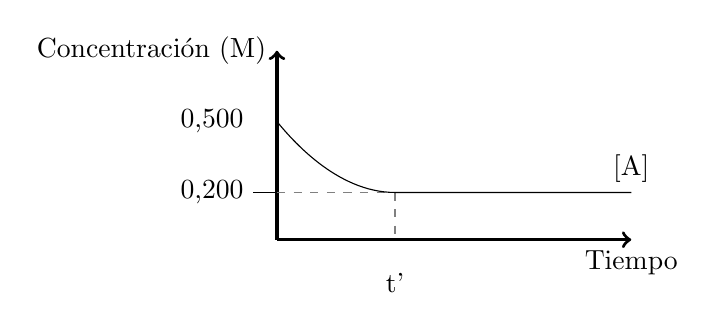
\begin{tikzpicture}[scale=3]
                  \coordinate (t) at (0.5,0);
                  \coordinate (A) at (1.5,0.2);
                  \coordinate (M) at (0,0.5);

                  % Ejes
                  \begin{scope}[very thick, ->]
                      \draw (0,0) -- (A |- 0,0) node[below]{Tiempo}; % X
                      \draw (0,0) -- (0,0.8) node[left]{Concentración (M)}; % Y
                  \end{scope}

                  % Ref
                  \draw (0,0 |- A) -- +(-0.1,0) node[left]{\num{0,200}};
                  \draw (M) +(-0.1,0) node[left]{\num{0,500}};
                  \draw (t) +(0,-0.1) node[below]{t'};
                  \draw (t |- A) -- (A) node[above]{[A]};

                  % Guias
                  \begin{scope}[dashed, thin, gray]
                      \draw (0,0 |- A) -- (t |- A); % 0,200 ---
                      \draw (t |- A) -- (t |- 0,0); % r |
                  \end{scope}

                  % Gráfico
                  \begin{scope}
                      \draw (M) parabola[bend at end] (t |- A) -- (A);
                  \end{scope}
              \end{tikzpicture}
          \end{figure}

    \item[5.] En un recipiente de \SI{500}{\cm\cubed}, a determinada temperatura, se colocan \SI{0,500}{\mole} de
          $NOCl \eg$; \SI{0,500}{\mole} de $NO \eg$ y \SI{0,250}{\mole} de $Cl_2 \eg$. La ecuación que representa la
          reacción es:
          \[ 2 NO \eg + Cl_2 \eg \llra 2 NOCl \eg \]
          Dato: $Kc$ (T) = \num{85,7}

          Indiquen:
          \begin{enumerate}
              \item si el sistema se encuentra en equilibrio o, de lo contrario, en qué sentido evoluciona para alcanzarlo;
              \item cuál de las siguientes opciones se cumple antes de que el sistema alcance el equilibrio:
                    \begin{enumerate}
                        \item $Kc < Qc$
                        \item $Kc > Qc$
                        \item $Kc = Qc$
                        \item $Qc < 0$
                    \end{enumerate}
          \end{enumerate}

    \item[7.] Los siguientes esquemas representan la composición de dos sistemas. Los dos recipientes
          tienen el mismo volumen y se encuentran a la misma temperatura $T$.

          \begin{figure}[h]
              \begin{subfigure}{0.5\textwidth}
                  % "molecula" está definido en el preambulo de este archivo
                  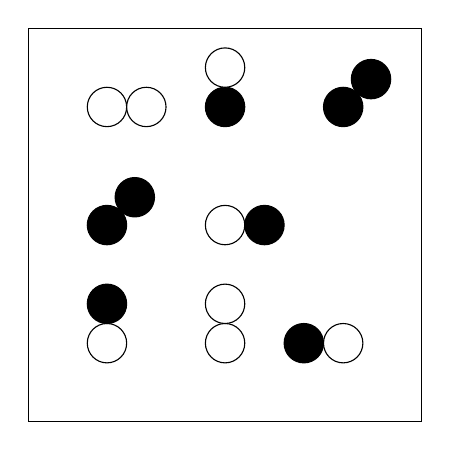
\begin{tikzpicture}
                      \draw (0,0) rectangle +(5,5);
                      \pic[shift={(1,4)}]{molecula=white/white};
                      \pic[shift={(2.5,4)},rotate=90]{molecula=black/white};
                      \pic[shift={(4,4)},rotate=45]{molecula=black/black};

                      \pic[shift={(1,2.5)},rotate=45]{molecula=black/black};
                      \pic[shift={(2.5,2.5)}]{molecula=white/black};

                      \pic[shift={(1,1)},rotate=90]{molecula=white/black};
                      \pic[shift={(2.5,1)},rotate=90]{molecula=white/white};
                      \pic[shift={(3.5,1)}]{molecula=black/white};
                  \end{tikzpicture}

                  \caption{}
              \end{subfigure}
              \begin{subfigure}{0.5\textwidth}
                  % "molecula" está definido en el preambulo de este archivo
                  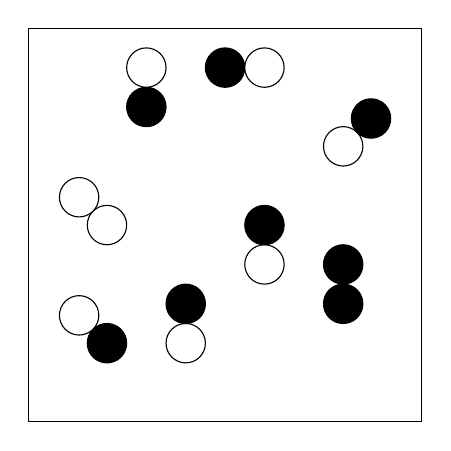
\begin{tikzpicture}
                      \draw (0,0) rectangle +(5,5);
                      \pic[shift={(1.5,4)},rotate=90]{molecula=black/white};
                      \pic[shift={(2.5,4.5)}]{molecula=black/white};
                      \pic[shift={(4,3.5)},rotate=45]{molecula=white/black};

                      \pic[shift={(1,2.5)},rotate=135]{molecula=white/white};

                      \pic[shift={(1,1)},rotate=135]{molecula=black/white};
                      \pic[shift={(2,1)},rotate=90]{molecula=white/black};
                      \pic[shift={(3,2)},rotate=90]{molecula=white/black};
                      \pic[shift={(4,1.5)},rotate=90]{molecula=black/black};

                  \end{tikzpicture}

                  \caption{}
              \end{subfigure}
          \end{figure}
          \begin{itemize}
              \item[\circ] Representa un átomo de $A$
              \item[\bullet] Representa un átomo de $J$
          \end{itemize}

          El número de moléculas dibujadas es proporcional a la cantidad de moléculas, expresada en
          moles.
          El valor de la constante de equilibrio Kc de la descomposición de $AJ$ a la temperatura $T$ es
          de \num{0,25}.
          \begin{enumerate}
              \item Escriban la ecuación que representa la reacción.
              \item Identifiquen si los sistemas se encuentran en equilibrio o, de lo contrario, en qué sentido
                    evolucionan para alcanzarlo.
          \end{enumerate}

    \item[8.] La descomposición del $SO_3$ es una reacción endotérmica. La ecuación que representa el
          proceso es:
          \[ 2 SO_3 \eg \llra O_2 \eg + 2 SO_2 \eg \]
          Indiquen cómo variar los siguientes factores para aumentar el rendimiento de la reacción:
          \begin{enumerate}
              \item temperatura;
              \item presión;
              \item cantidad de oxígeno;
              \item cantidad de $SO_3$.
          \end{enumerate}

    \item[9.] Las siguientes ecuaciones representan reacciones reversibles:
          \begin{enumerate}
              \item \[ C_2H_4 \eg + Cl_2 \eg \xleftrightarrow[Exotérmica]{Endotérmica} C_2H_4Cl_2 \]
              \item \[ N_2 \eg + O_2 \eg \xleftrightarrow[Exotérmica]{Endotérmica} 2 NO \eg \]
          \end{enumerate}
          Predigan el efecto provocado sobre las concentraciones de los productos y el valor de la
          constante de equilibrio de cada reacción, para cada uno de los siguientes cambios:
          \begin{enumerate}
              \item se reduce el volumen del recipiente (temperatura constante);
              \item se eleva la temperatura del sistema;
              \item se agrega uno de los reactivos (temperatura constante).
          \end{enumerate}

\end{enumerate}
\end{document}